\documentclass[aspectratio=169,11pt,fontset=none]{ctexbeamer}

\usetheme{Madrid}
\usecolortheme{default}
\setbeamertemplate{navigation symbols}{}
\setbeameroption{hide notes}
\usepackage{tikz}
\usetikzlibrary{arrows.meta,fit,positioning}

\setCJKmainfont{NotoSansCJKsc-Regular.otf}[Path=fonts/,BoldFont=NotoSansCJKsc-Bold.otf]
\setCJKsansfont{NotoSansCJKsc-Regular.otf}[Path=fonts/,BoldFont=NotoSansCJKsc-Bold.otf]

\definecolor{HustBlue}{RGB}{22,87,170}
\definecolor{HustTeal}{RGB}{0,122,128}
\definecolor{HustOrange}{RGB}{204,102,0}
\definecolor{HustGray}{RGB}{72,72,72}
\definecolor{HustLight}{RGB}{245,247,250}
\definecolor{SurveyBlue}{HTML}{E6F0FA}
\definecolor{SurveyGreen}{HTML}{E9F5EE}
\definecolor{SurveyOrange}{HTML}{FCEFE3}
\definecolor{SurveyGray}{HTML}{F2F3F5}
\definecolor{SurveyRed}{HTML}{F7E6E6}

\setbeamercolor{title}{fg=white,bg=HustBlue}
\setbeamercolor{frametitle}{fg=white,bg=HustBlue}
\setbeamercolor{structure}{fg=HustBlue}
\setbeamercolor{block title}{fg=white,bg=HustBlue}
\setbeamercolor{block body}{fg=black,bg=HustLight}
\setbeamercolor{alerted text}{fg=HustOrange}
\setbeamerfont{title}{series=\bfseries,size=\LARGE}
\setbeamerfont{frametitle}{series=\bfseries}

\setbeamertemplate{footline}{%
  \leavevmode%
  \hbox{%
    \begin{beamercolorbox}[wd=.8\paperwidth,ht=2.5ex,dp=1ex,leftskip=1em]{author in head/foot}%
      \color{HustGray}vLLM-HUST\hfill 国产算力与 AGI4S 推理底座
    \end{beamercolorbox}%
    \begin{beamercolorbox}[wd=.2\paperwidth,ht=2.5ex,dp=1ex,center]{date in head/foot}%
      \insertframenumber{} / \inserttotalframenumber
    \end{beamercolorbox}%
  }%
  \vskip0pt%
}

\title{vLLM-HUST 介绍}
\subtitle{面向国产算力与 AGI4S 场景的可演进推理底座}
\author{HUST 团队}
\date{二〇二六年五月}

\newcommand{\HuaweiAscend}{华为昇腾}

\begin{document}

\begin{frame}[plain]
  \titlepage
  \note{本报告内容整理依据包括 vllm-hust 系列仓库源码、架构文档与实施方案材料。}
\end{frame}

\begin{frame}{汇报提纲}
  \tableofcontents
\end{frame}

\section{定位与背景}

\begin{frame}{项目定位}
  \begin{block}{vLLM-HUST 是什么}
    vLLM-HUST 以 upstream vLLM 为基础，围绕\alert{国产算力适配}、\alert{AGI4S 服务场景}与\alert{benchmark 驱动验证}建设可持续演进的推理系统底座。
  \end{block}

  \vspace{0.6em}
  \begin{columns}[T]
    \column{0.48\textwidth}
    \begin{block}{目标}
      \begin{itemize}
        \item 保持与 upstream 的持续合并能力
        \item 支撑国产硬件上的高吞吐、低时延、低成本服务
        \item 为多模态、智能体、工具调用和长上下文提供统一底座
      \end{itemize}
    \end{block}

    \column{0.48\textwidth}
    \begin{block}{方法}
      \begin{itemize}
        \item 插件优先，缩小 fork 差异面
        \item 平台隔离，避免共享热路径散落硬件分支
        \item 用真实 workload 评估，而非只看微基准
      \end{itemize}
    \end{block}
  \end{columns}
\end{frame}

\begin{frame}{为什么需要 vLLM-HUST}
  \begin{columns}[T]
    \column{0.52\textwidth}
    \begin{block}{场景牵引}
      \begin{itemize}
        \item 国产硬件环境下，推理执行图、通信运行时与多级存储协同优化难度高
        \item AGI4S、多模态智能体、行业级 RAG 要求同时满足长上下文、工具调用和流式交互
        \item 真实交付还需要部署、修复、指标、展示和回归闭环
      \end{itemize}
    \end{block}

    \column{0.44\textwidth}
    \begin{alertblock}{核心矛盾}
      \begin{itemize}
        \item 软硬协同难
        \item KV 状态难管理
        \item 异构互联难提效
        \item 性能收益难被稳定证明
      \end{itemize}
    \end{alertblock}
  \end{columns}

  \vspace{0.5em}
  \centering
  \textbf{建设重点：}在保持主干可持续演进的前提下，将国产算力需求与复杂场景需求落实到可维护、可验证的扩展边界。
\end{frame}

\section{系列仓库}

\begin{frame}{系列仓库版图}
  \small
  \begin{tabular}{p{0.27\textwidth}p{0.66\textwidth}}
    \textbf{仓库} & \textbf{职责} \\
    \hline
    vllm-hust & 主推理运行时，围绕 upstream vLLM 做可持续合并的增强 \\
    vllm-ascend-hust & Ascend 平台插件与 NPU 侧实现，隔离硬件特化逻辑 \\
    ascend-runtime-manager & Ascend 运行时诊断、环境修复、容器化与一键启动入口 \\
    vllm-hust-workstation & 本地工作站，聚合聊天、监控、外部应用接入与演示栈管理 \\
    vllm-hust-website & 官网、版本元数据、workstation 嵌入与 leaderboard 展示 \\
    vllm-hust-benchmark & benchmark wrapper、结果导出与 website 聚合入口 \\
    vllm-hust-docs & 架构拆解、运维指南、同步记录与对外介绍材料 \\
    EvoScientist & 外部多智能体真实业务负载，用于验证 agent 场景承载能力 \\
  \end{tabular}
\end{frame}

\begin{frame}{端到端协同链}
  \begin{columns}[T]
    \column{0.48\textwidth}
    \begin{block}{入口层}
      \begin{itemize}
        \item OpenAI-compatible API
        \item workstation Web 交互界面
        \item 外部多智能体 workload 接入
        \item website 与 docs 展示入口
      \end{itemize}
    \end{block}

    \begin{block}{运行时层}
      \begin{itemize}
        \item CLI / API / offline 推理入口
        \item V1 engine、EngineCore、executor、worker
        \item model registry、loader、KV cache、quantization、compilation
      \end{itemize}
    \end{block}

    \column{0.48\textwidth}
    \begin{block}{平台与治理层}
      \begin{itemize}
        \item platform interface + plugin discovery
        \item Ascend plugin 独立演进
        \item runtime manager 负责环境修复与容器工作流
      \end{itemize}
    \end{block}

    \begin{block}{验证与发布层}
      \begin{itemize}
        \item benchmark wrapper 统一实验入口
        \item artifact 聚合到 website leaderboard
        \item docs 持续沉淀架构与运维知识
      \end{itemize}
    \end{block}
  \end{columns}
\end{frame}

\section{技术架构}

\begin{frame}{vLLM-HUST 核心架构分层}
  \small
  \begin{tabular}{p{0.2\textwidth}p{0.72\textwidth}}
    \textbf{分层} & \textbf{主要内容} \\
    \hline
    接口与入口层 & CLI、OpenAI 兼容服务、离线推理入口 \\
    参数与配置层 & EngineArgs、VllmConfig，以及 model/cache/parallel/multimodal 等 schema \\
    请求编排层 & renderer、input processor、output processor、流式生命周期管理 \\
    引擎核心层 & V1 LLMEngine、EngineCore、调度、连续批处理与 core 通信 \\
    模型执行层 & model registry、model loader、worker、runner、layers、kernels \\
    平台与插件层 & platform interface、builtin detectors、platform plugins、general plugins \\
    横切能力层 & multimodal、reasoning、tool parser、structured outputs、renderers \\
    性能基础设施层 & KV cache、quantization、compilation、distributed、profiling、tracing \\
  \end{tabular}

  \vspace{0.6em}
  \begin{alertblock}{设计原则}
    面向国产硬件和复杂场景的差异化需求，通过分层抽象、平台接口与插件机制分别归入合适的实现边界。
  \end{alertblock}
\end{frame}

\begin{frame}{vLLM-HUST 的推理执行全景}
  \centering
  \resizebox{0.96\linewidth}{!}{\definecolor{DiagramBlue}{HTML}{E6F0FA}
\definecolor{DiagramGreen}{HTML}{E9F5EE}
\definecolor{DiagramOrange}{HTML}{FCEFE3}
\definecolor{DiagramGray}{HTML}{F2F3F5}
\begin{tikzpicture}[
    node distance=9mm and 12mm,
    scale=1.0,
    transform shape,
    block/.style={draw=black!70, line width=0.85pt, rounded corners=2.4pt, align=center, minimum height=11.5mm, inner sep=4.5pt, font=\normalsize\sffamily},
    group/.style={draw=black!55, line width=0.8pt, rounded corners=3pt, inner sep=7pt},
    note/.style={font=\small\sffamily, align=center, fill=white, inner sep=1.8pt, text=black!75},
    flow/.style={-{Latex[length=3.2mm,width=2.1mm]}, line width=0.9pt, draw=black!75}
]
\node[block, fill=DiagramGray, minimum width=3.3cm] (ingress) {\textbf{复杂请求入口}\\文本/长上下文/多模态/工具调用};
\node[block, fill=DiagramBlue, minimum width=3.1cm, right=of ingress] (service) {\textbf{服务入口}\\OpenAI 兼容/API/监控};
\node[block, fill=DiagramBlue, minimum width=3.1cm, right=of service] (scheduler) {\textbf{请求调度}\\批处理组织/SLO/回退};

\node[block, fill=DiagramGreen, minimum width=2.8cm, below=12mm of service, xshift=-8mm] (execute) {\textbf{模型执行}\\prefill/decode/并行策略};
\node[block, fill=DiagramGreen, minimum width=2.8cm, right=of execute] (cache) {\textbf{KV 状态管理}\\前缀复用/迁移/驱逐};
\node[block, fill=DiagramGreen, minimum width=2.8cm, right=of cache] (backend) {\textbf{平台后端接口}\\图模式/算子/能力门控};
\node[group, fit=(execute)(cache)(backend), label={[font=\small\sffamily\bfseries, fill=white, inner sep=1.5pt]below:运行时核心}] (runtime) {};

\node[block, fill=DiagramOrange, minimum width=3.0cm, below=12mm of cache, xshift=-8mm] (compiler) {\textbf{平台运行时}\\CANN/插件栈/通信};
\node[block, fill=DiagramOrange, minimum width=2.7cm, below=10mm of compiler] (device) {\textbf{国产硬件平台}\\NPU/GPU/驱动};
\node[group, fit=(compiler)(device), label={[font=\small\sffamily\bfseries, fill=white, inner sep=1.5pt]below:平台边界}] (platform) {};

\draw[flow] (ingress) -- (service);
\draw[flow] (service) -- (scheduler);
\draw[flow] (scheduler) -- (execute);
\draw[flow] (scheduler) -- (cache);
\draw[flow] (scheduler) -- (backend);
\draw[flow] (execute) -- (cache);
\draw[flow] (cache) -- (backend);
\draw[flow] (backend) -- (compiler);
\draw[flow] (compiler) -- (device);
\draw[flow] (device.east) -| ([xshift=12mm]backend.east) -- (backend.east);
\draw[flow, dashed, line width=0.8pt, draw=black!65] (cache.south) -- ++(0,-8mm) -| ([xshift=-10mm]execute.west) -- ++(0,12mm) -| ([yshift=-6mm]service.south) -- (service.south);

\node[note, text width=4.0cm, right=10mm of scheduler] {复杂请求首先考验入口编排与调度策略};
\node[note, text width=4.0cm, right=10mm of device] {硬件差异应尽量收敛在平台接口与运行时边界};
\end{tikzpicture}}
\end{frame}

\begin{frame}{总图对应到 vLLM-HUST 的三层实现边界}
  \small
  \begin{block}{服务入口与调度层}
    OpenAI 兼容入口、workstation 接入、请求编排、连续批处理和流式生命周期管理，决定请求如何进入系统并被组织执行。
  \end{block}

  \begin{block}{执行与后端边界}
    model registry、loader、worker、runner、KV cache、quantization、compilation 与 platform interface 共同决定请求如何被真正执行，以及不同后端能力如何被接入。
  \end{block}

  \begin{alertblock}{平台与治理层}
    runtime manager、CANN/torch\_npu、容器工作流和 benchmark 回归链路负责把硬件差异、环境修复和交付验证限制在可维护边界内。
  \end{alertblock}
\end{frame}

\begin{frame}{国产硬件适配路径：保持主干可合并性}
  \begin{columns}[T]
    \column{0.5\textwidth}
    \begin{block}{主仓库负责的边界}
      \begin{itemize}
        \item env override：import 前最小环境补齐
        \item CLI 预检：尽早发现 torch\_npu / runtime 问题
        \item platform interface：平台能力抽象与后端选择
        \item plugin discovery：外部硬件实现的标准挂载点
      \end{itemize}
    \end{block}

    \column{0.5\textwidth}
    \begin{block}{当前重点平台与扩展方向}
      \begin{itemize}
        \item 当前主要适配：\HuaweiAscend、沐曦、海光、百度昆仑芯
        \item 当前重点放在\HuaweiAscend，但架构不绑定单一硬件路线
        \item 平台插件、runtime manager、benchmark 共同支撑后续平台扩展
      \end{itemize}
    \end{block}
  \end{columns}

  \vspace{0.5em}
  \centering
  \alert{效果：主干差异范围更可控，硬件特化逻辑可独立演进、独立验证和独立回归。}
\end{frame}

\begin{frame}{vLLM-HUST 的演进主线}
  \centering
  \resizebox{0.9\linewidth}{!}{\definecolor{FocusBlue}{HTML}{E6F0FA}
\definecolor{FocusGreen}{HTML}{E9F5EE}
\definecolor{FocusOrange}{HTML}{FCEFE3}
\definecolor{FocusGray}{HTML}{F2F3F5}
\definecolor{FocusRed}{HTML}{F7E6E6}
\begin{tikzpicture}[
    node distance=16mm and 20mm,
    scale=1.05,
    transform shape,
    block/.style={draw=black!70, line width=0.85pt, rounded corners=2.4pt, minimum width=33mm, minimum height=11mm, align=center, font=\normalsize\sffamily, inner sep=4.5pt},
    centerblock/.style={draw=black!70, line width=0.9pt, rounded corners=3pt, minimum width=42mm, minimum height=13mm, align=center, font=\normalsize\sffamily\bfseries, inner sep=5pt},
    note/.style={font=\small\sffamily, align=center, fill=white, inner sep=1.6pt, text=black!75},
    flow/.style={-{Latex[length=3.0mm,width=2.0mm]}, line width=0.9pt, draw=black!75}
]
\node[centerblock, fill=FocusGray] (goal) {\textbf{vLLM-HUST 持续演进的}\\\textbf{推理底座}};

\node[block, fill=FocusBlue, above left=18mm and 26mm of goal] (plugin) {\textbf{平台插件化}\\抽象边界/注册表/可合并优化};
\node[block, fill=FocusGreen, above right=18mm and 26mm of goal] (runtime) {\textbf{调度与状态治理}\\SLO/KV Cache/迁移/回退};
\node[block, fill=FocusOrange, below left=18mm and 26mm of goal] (eval) {\textbf{统一评测闭环}\\近真实负载/成本/稳定性指标};
\node[block, fill=FocusRed, below right=18mm and 26mm of goal] (model) {\textbf{复杂场景承载}\\多模态/工具调用/reasoning};

\draw[flow] (plugin.south east) -- (goal.north west);
\draw[flow] (runtime.south west) -- (goal.north east);
\draw[flow] (eval.north east) -- (goal.south west);
\draw[flow] (model.north west) -- (goal.south east);

\node[note, text width=7.6cm, above=6mm of goal] {真正可持续的优势，不来自单点优化，而来自多条能力线同步推进。};
\node[note, text width=7.6cm, below=6mm of goal] {目标是让系统同时具备可合并、可验证、可交付和可持续优化能力。};
\end{tikzpicture}}

\end{frame}

\begin{frame}{当前建设重点}
  \small
  \begin{columns}[T]
    \column{0.48\textwidth}
    \begin{block}{后端插件化}
      用 vllm-hust 与 vllm-ascend-hust 的分层保持 merge-safe，尽量不把硬件特化逻辑散落到共享热路径。
    \end{block}

    \begin{block}{资源管理与调度}
      围绕 SLO、KV cache、迁移、回退与阶段解耦，解决真实业务负载下的吞吐与稳定性问题。
    \end{block}

    \column{0.48\textwidth}
    \begin{block}{统一评测与观测}
      通过 benchmark、website、docs 和 artifact 元数据形成持续回归与对外展示闭环。
    \end{block}

    \begin{block}{模型结构演进}
      让底座持续承接多模态、工具调用、reasoning 和语音交互等复杂请求形态。
    \end{block}
  \end{columns}

\end{frame}

\begin{frame}{AGI4S 能力链：输入、执行、输出一体化}
  \begin{columns}[T]
    \column{0.32\textwidth}
    \begin{block}{输入侧}
      \begin{itemize}
        \item chat template / renderer
        \item multimodal registry
        \item 多模态预算与预处理
      \end{itemize}
    \end{block}

    \column{0.32\textwidth}
    \begin{block}{执行侧}
      \begin{itemize}
        \item continuous batching
        \item 长上下文与 KV cache 管理
        \item streaming 与 structured outputs
      \end{itemize}
    \end{block}

    \column{0.32\textwidth}
    \begin{block}{输出侧}
      \begin{itemize}
        \item reasoning parser
        \item tool parser
        \item OpenAI 兼容响应装配
      \end{itemize}
    \end{block}
  \end{columns}

  \vspace{0.7em}
  \begin{itemize}
    \item 当前结构已将多模态、reasoning、tool calling 纳入核心能力体系。
    \item 因而 vLLM-HUST 能够支撑多智能体、科研自动化和复杂交互 workload。
  \end{itemize}
\end{frame}

\section{工程交付}

\begin{frame}{工程化交付链路}
  \small
  \begin{columns}[T]
    \column{0.48\textwidth}
    \begin{block}{对外入口}
      \begin{itemize}
        \item workstation 负责本地交互、监控面板、外部应用接入和演示控制
        \item website 负责项目展示、版本元数据、workstation 嵌入和 benchmark 榜单
      \end{itemize}
    \end{block}

    \begin{block}{运行时治理}
      \begin{itemize}
        \item runtime repair、container、ssh-deploy 提供标准化运行时治理入口
        \item 把环境修复、诊断和容器化从模型执行热路径中拆开管理
      \end{itemize}
    \end{block}

    \column{0.48\textwidth}
    \begin{block}{实验与回归}
      \begin{itemize}
        \item benchmark wrapper 提供统一实验入口，结果导出为 leaderboard artifact 与 manifest
        \item website 聚合结果，docs 负责架构、操作和长期介绍材料沉淀
      \end{itemize}
    \end{block}

    \begin{alertblock}{一句话概括}
      vLLM-HUST 不只是推理内核，还把运行、验证、展示和知识沉淀串成一条完整交付链路。
    \end{alertblock}
  \end{columns}
\end{frame}

\begin{frame}{workstation 工作台实景}
  \centering
  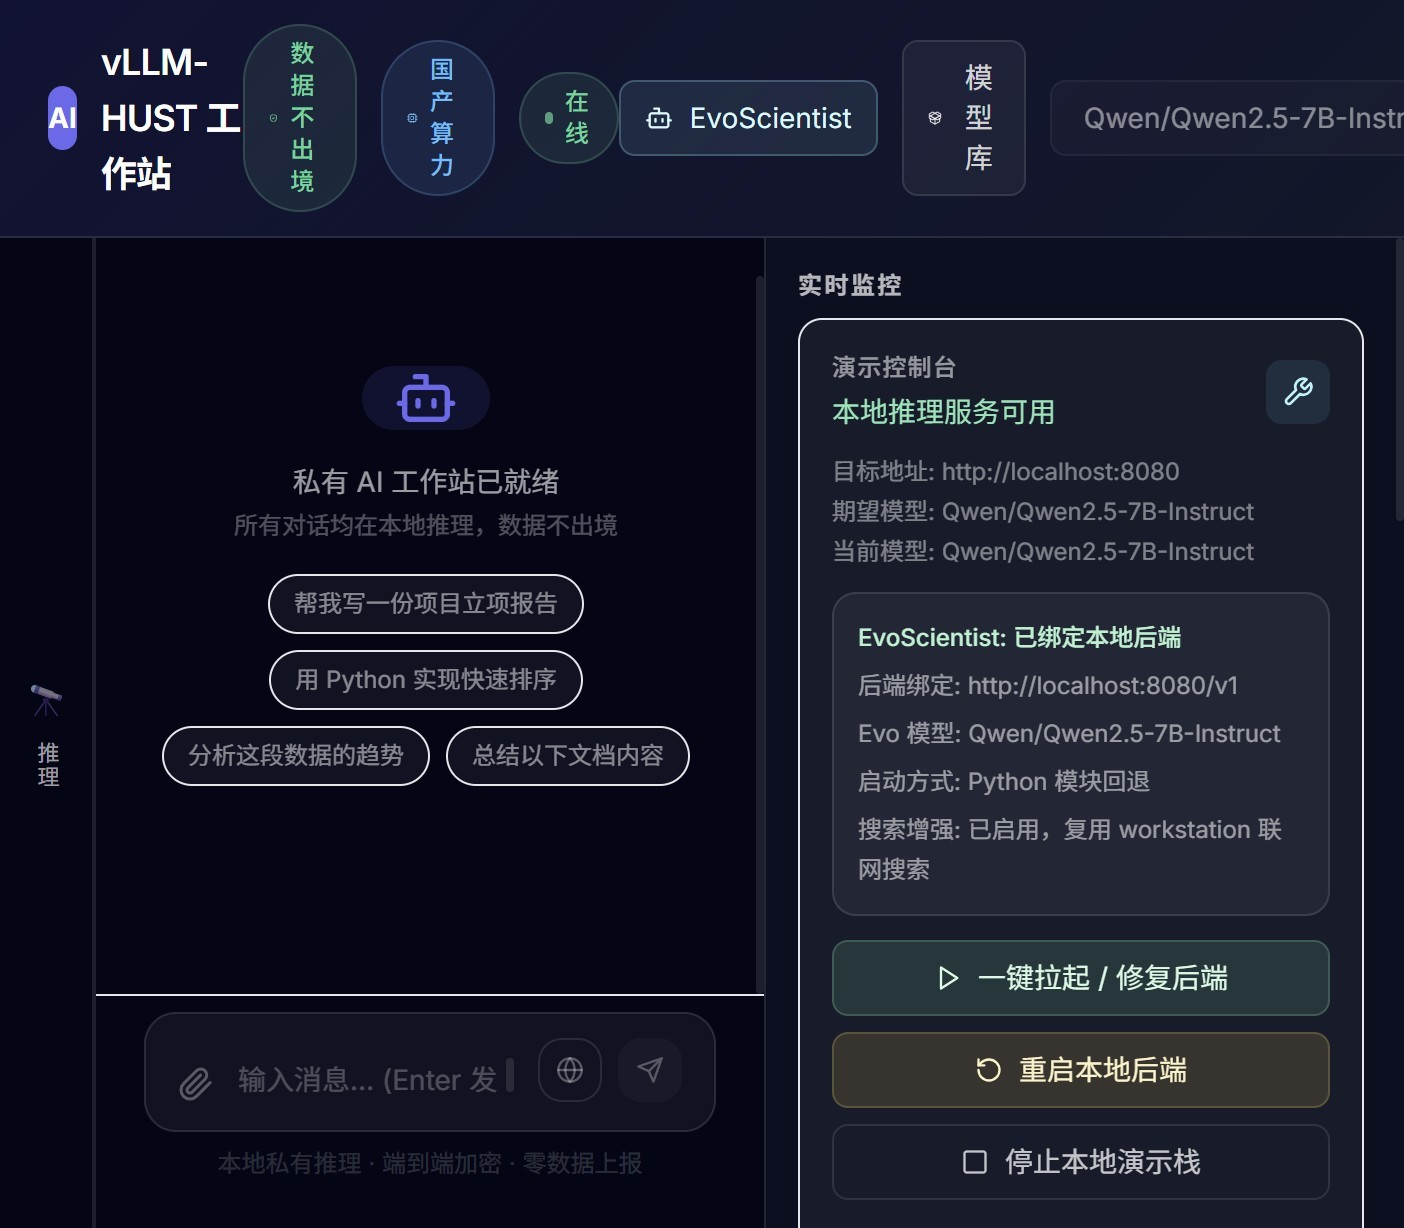
\includegraphics[width=0.96\linewidth,height=0.78\textheight,keepaspectratio]{assets/workstation-dashboard.jpg}

  \vspace{0.25em}
  {\small 用于演示控制、状态观察、外部应用接入和本地交互。}
\end{frame}

\section{进展与路线}

\begin{frame}{当前阶段判断}
  \small
  \begin{block}{已经基本明确的部分}
    \begin{itemize}
      \item 底层路线已经清晰：以 merge-safe 的平台分层承接国产硬件差异，以统一推理底座承接复杂场景需求。
      \item 关键能力已经成形：多模态、流式输出、reasoning、tool calling 和 structured outputs 已具备服务化承载基础。
      \item 工程闭环已经打通：运行、验证、展示和文档沉淀不再割裂，能够支撑持续演进与对外说明。
    \end{itemize}
  \end{block}

  \begin{alertblock}{当前仍需重点补强的部分}
    \begin{itemize}
      \item 更接近真实业务的多智能体与长链路 workload 验证。
      \item 跨硬件、跨配置、跨阶段的一致性回归与稳定性证明。
    \end{itemize}
  \end{alertblock}
\end{frame}

\begin{frame}{验证与度量闭环}
  \small
  \begin{columns}[T]
    \column{0.48\textwidth}
    \begin{block}{关键指标}
      \begin{itemize}
        \item TTFT、ITL、TPOT、吞吐、token 速率
        \item 长上下文稳定性、多租户利用率、工具调用链路质量
      \end{itemize}
    \end{block}

    \begin{block}{实验入口与产物}
      \begin{itemize}
        \item vllm bench serve / throughput / latency
        \item wrapper 仓库统一提供 run / run-both / export / publish 入口
        \item benchmark 结果导出为 leaderboard artifact 与 manifest
      \end{itemize}
    \end{block}

    \column{0.48\textwidth}
    \begin{block}{展示与回归}
      \begin{itemize}
        \item website 聚合结果并持续展示横向对比
        \item docs 解释指标口径、测试入口和阶段结论
        \item 统一度量体系为国产硬件适配与 AGI4S 优化提供共同证据
      \end{itemize}
    \end{block}
  \end{columns}
\end{frame}

\begin{frame}{benchmark 榜单快照}
  \small
  \begin{columns}[T,onlytextwidth]
    \column{0.76\textwidth}
    \centering
    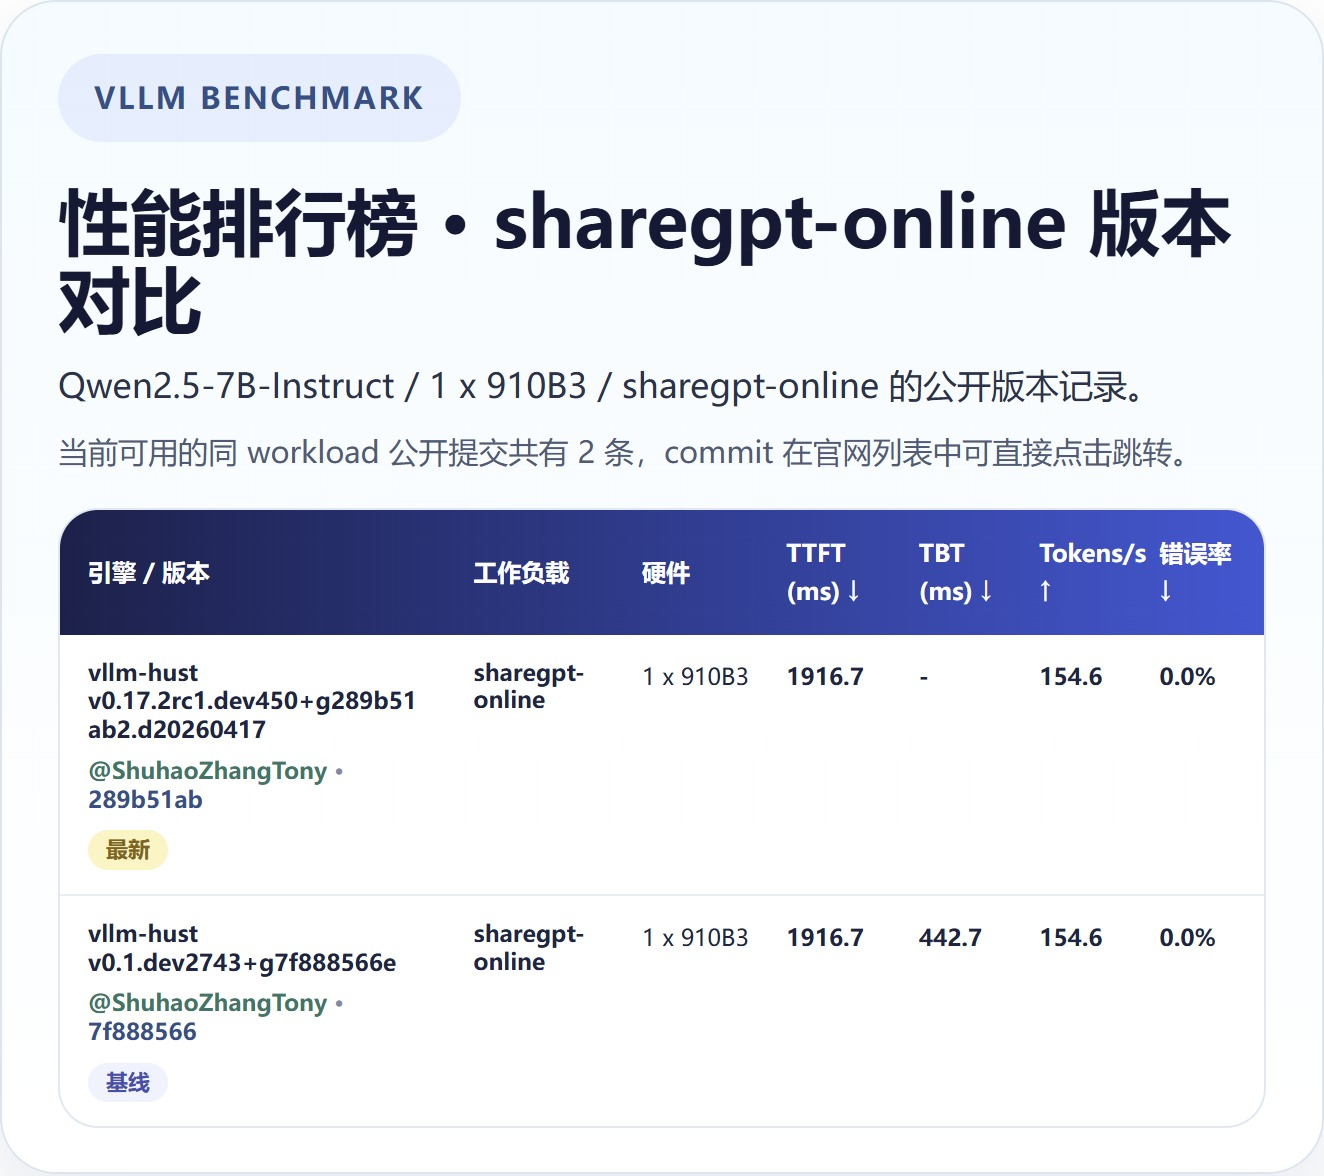
\includegraphics[width=\linewidth,height=0.76\textheight,keepaspectratio]{assets/website-leaderboard.jpg}

    \column{0.22\textwidth}
    \begin{block}{同一 workload 版本对比}
      \scriptsize
      这一页不再混放不同 workload，而是收敛到同模型、同硬件、同 workload 的公开提交结果。

      当前本地快照中，可直接对比的 sharegpt-online 单机单卡样本共有 2 条。

      可点击提交：\\
      \href{https://github.com/vLLM-HUST/vllm-hust/commit/289b51ab21d6f27abc043fd5917761b62c039871}{289b51ab}\\
      \href{https://github.com/vLLM-HUST/vllm-ascend-hust/commit/7f888566e7209ff8fe417f79c3a691354301ac9f}{7f888566}
    \end{block}
  \end{columns}

\end{frame}

\begin{frame}{核心贡献者快照}
  \small
  \begin{columns}[T,onlytextwidth]
    \column{0.76\textwidth}
    \centering
    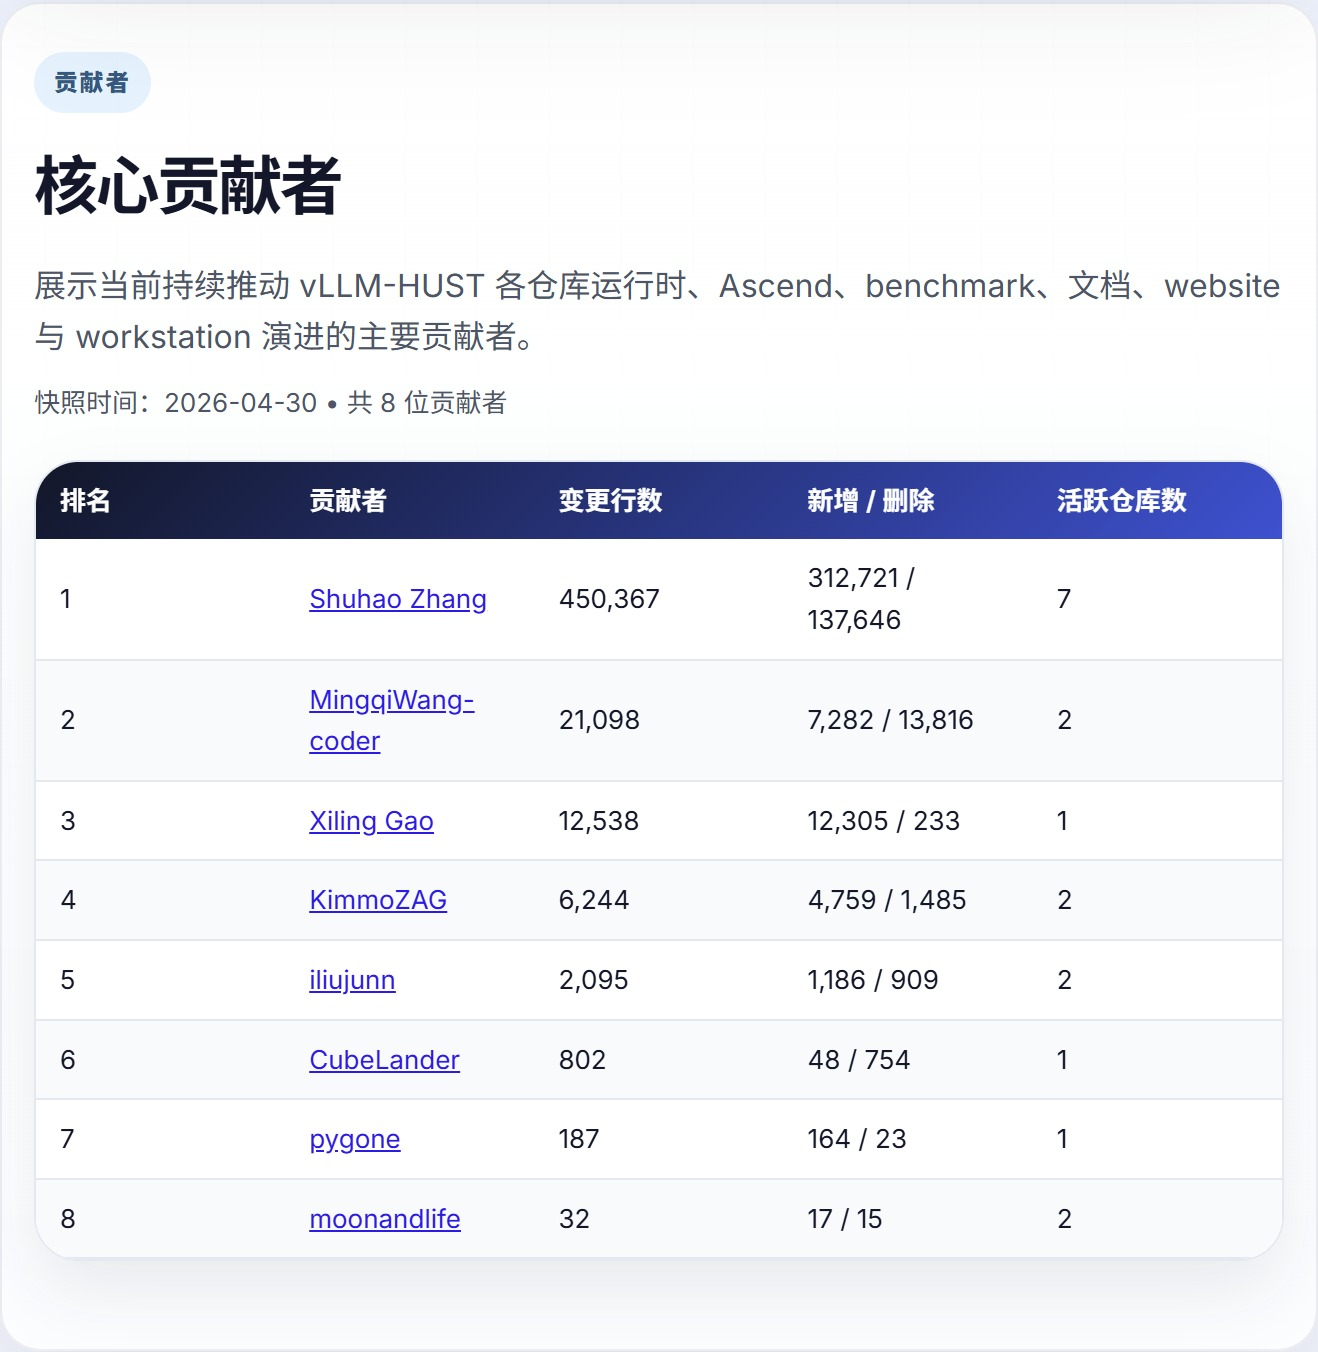
\includegraphics[width=\linewidth,height=0.76\textheight,keepaspectratio]{assets/core-contributors.jpg}

    \column{0.22\textwidth}
    \begin{block}{持续建设这套底座的人}
      \footnotesize
      官网持续聚合系列仓库的贡献者快照。

      这一页可以直观看到当前哪些人正在推进运行时、Ascend 适配、benchmark、文档、website 与 workstation 的协同演进。
    \end{block}
  \end{columns}
\end{frame}

\begin{frame}{研发队伍与成果落地机制}
  \small
  \begin{columns}[T]
    \column{0.48\textwidth}
    \begin{block}{核心代码与适配队伍}
      \begin{itemize}
        \item 持续研究 vllm-hust 核心代码、执行链和平台抽象
        \item 面向国产硬件做适配策略、插件接入和运行时治理
        \item 先聚焦\HuaweiAscend，同时保留对其他国产平台的扩展能力
      \end{itemize}
    \end{block}

    \column{0.48\textwidth}
    \begin{block}{性能优化队伍}
      \begin{itemize}
        \item 独立推进吞吐、时延、长上下文与算子路径优化
        \item 优化成果以平台能力形式沉淀回 vllm-hust
        \item 目标是将优化成果沉淀为平台能力，并在国产硬件上稳定复用
      \end{itemize}
    \end{block}
  \end{columns}

  \vspace{0.5em}
  \begin{alertblock}{组织机制}
    适配工作与性能优化工作通过统一平台持续汇聚，最终沉淀为可复用、可验证、可扩展的国产算力能力体系。
  \end{alertblock}
\end{frame}

\begin{frame}{下一阶段重点}
  \small
  \begin{enumerate}
    \item 继续把硬件差异约束在平台插件、运行时治理和验证配置层，维持主干可持续演进。
    \item 围绕多智能体、长上下文、工具调用和多模态交互，补齐近真实业务压力下的系统性验证。
    \item 统一 workload schema、指标口径和实验元数据，让不同平台、不同配置下的结果可以稳定比较。
    \item 持续同步架构、操作和介绍材料，确保代码演进、验证结论和对外表达保持一致。
  \end{enumerate}

  \begin{block}{阶段目标}
    从“可以运行”进一步走向“可以交付、可以验证、可以持续优化”的国产推理底座。
  \end{block}
\end{frame}

\begin{frame}[plain]
  \vfill
  \centering
  \Large 谢谢
  \note{参考材料包括：vllm-hust README 与主仓代码结构；vllm-hust-docs/architecture 下的源码解构、平台链与 AGI4S 能力文档；课题实施方案材料与阶段汇报文稿；workstation、website、ascend-runtime-manager、benchmark 与外部验证 workload 各仓 README。}
\end{frame}

\end{document}